\section{Ingestion}

\subsection{Datenquelle}

Bei der Implementierung 

\begin{figure}
    \centering
    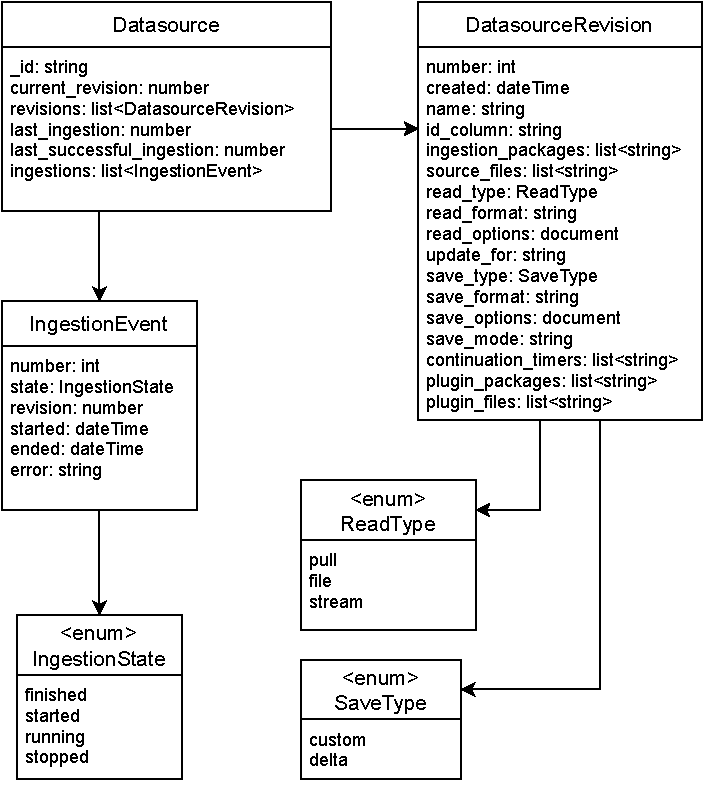
\includegraphics{Grafiken/ingestion-Datamodel.pdf}
    \caption{Datenmodell der Datenquelle}
    \label{fig:datasource_model}
\end{figure}

\subsection{Api-Server}

Da auch das Masterprojekt eine REST-Schnittstelle hat, bietet es sich an, diesen Server so zu erweitern, dass er als Api-Server für das neue System fungiert.
Um die neuen Endpunkte in die aktuelle Lösung zu integrieren, werden die existierenden Pfade, bis auf die zur Authentifizierung, nach "`/api/v1/"' verschoben und die neuen unter "`/api/v2/"' eingefügt.
Auf Grund der Tatsache, dass das neue System mit einem eigenen Datenmodell arbeitet, ist damit die Integration bereits abgehandelt, es muss nur darauf geachtet werden, die Funktionen der beiden Versionen zu trennen.
Die Endpunkte werden mit ihren Funktionen, wie in \fref{sec:arch} beschrieben, implementiert.

Bei der Erstellung und dem Aktualisieren von Datenquellen werden jedes mal eine neue Revision 
Dabei muss besonders darauf geachtet werden, dass bei jeder Änderung einer \verb|Datasource| eine neue \verb|DatasourceRevision| angelegt wird.
Die Quell- oder Plugindateien werden zentral im \textit{HDFS} jeweils einem Unterordner pro Datenquelle abgelegt.
So sind die Dateien von überall aus erreichbar und können auch bei replizierten oder verteilten Microservices verwendet werden.


\subsection{Ingestion-Server}



\subsection{Continuation-Server}